\chapter{The AK-MCS method}
\label{ch:5}
One of the techniques used to deal with the high computational cost of MCS is to try to approximate the value taken by the performance function at the points of the sample, thus avoiding the costly task of evaluating this function at every point. AK-MCS, which stands for an active learning reliability method combining Kriging and Monte Carlo Simulation, is a method that performs such estimation by using a Gaussian Process Regression. The method is exposed in \citep{Echard2011}, on which this chapter is mostly based, together with \citep{RW}. \\

In this chapter, the procedure for performing regressions with Gaussian processes is first reviewed, then the steps to be followed during the method are described, and finally some application examples are shown.

\section{Preliminaries}
\subsection{Gaussian Identity of conditional distributions}
The joint probability density of the multivariate Gaussian distribution is given by:
\begin{equation}
  p(\bm{x}|\bm{m},\bm{\Sigma}) = (2\pi)^{D/2}|\bm{\Sigma}|^{-1/2}\exp{\left(-\frac{1}{2}(\bm{x}-\bm{m})^{T}\bm{\Sigma}^{-1}(\bm{x}-\bm{m})\right)}
\end{equation}
where $\bm{x}$ is a vector of length $D$, $\bm{m}$ is the mean vector, and $\bm{\Sigma}$ is the covariance matrix, which is symmetric and positive definite. To say that $\bm{x}$ follows a Gaussian distribution with mean  $\bm{m}$ and covariance $\bm{\Sigma}$ one writes $\bm{x} \sim \mathcal{N}(\bm{m}, \bm{\Sigma})$. \\

Let $\bm{x}$ and $\bm{y}$ be jointly Gaussian random vectors
\begin{equation}
  \begin{bmatrix}
    \bm{x} \\ \bm{y}
  \end{bmatrix}
  \sim \mathcal{N}\left(
    \begin{bmatrix}
    \bm{\mu_x} \\ \bm{\mu_y}
    \end{bmatrix} , \begin{bmatrix}
      \bm{A} & \bm{C} \\ \bm{C}^T & \bm{B}
    \end{bmatrix} \right)
\end{equation}

then the conditional distribution of $\bm{x}$ given $\bm{y}$ is:
\begin{equation} \label{eq:cond}
  \bm{x}|\bm{y} \sim \mathcal{N}\left(\bm{\mu_x} + \bm{C} \bm{B}^{-1}(\bm{y}-\bm{\mu_y}), \; \bm{A} - \bm{C}\bm{B}^{-1}\bm{C}^T \right)
\end{equation}
The proof of this fact can be detailed in \citep{Bishop}, section 3.1.

\subsection{Gaussian Process regression (or Kriging)}
A Gaussian process, is a collection of random variables, any finite number of which have a joint Gaussian distribution. It is completely specified by its mean function and covariance function. To say that a real process $f(\bm{x})$ is Gaussian with mean function $m(\bm{x})$ and covariance function $k(\bm{x}, \bm{x'})$ one writes: 

\begin{equation}
  f(\bm{x}) \sim \mathcal{GP}(m(\bm{x}), k(\bm{x}, \bm{x'}))
\end{equation}

that is, every value of $f(\bm{x})$ at a location $\bm{x}$ is a random variable that follows a Gaussian distribution. Usually, for simplicity of notation, the mean function is considered to be zero. \\

Gaussian processes can be used to make predictions. Let $(\bm{X}, \bm{\mathrm{f}}) = \{(\bm{x}_i, \mathrm{f}_i)|i \: = \: 1, \ldots, n\}$ be a set of observations (or training data) and $\bm{X}_*$ a set of $n_*$ input values for which we have to determine the value of $\mathrm{f}_*$ (or test data). Moreover, suppose that the observations $\mathrm{f}$ are noisy, i.e. the exact value of $\mathrm{f}$ is not known but that of $\bm{y} = \bm{\mathrm{f}} + \bm{\epsilon}$. Assuming that the noise $\bm{\epsilon}$ is additive independent identically Gaussian distributed with variance $\sigma_n^2$, the covariance on the observations becomes
\begin{equation}
  \text{cov}(y_p, y_q) = k(\bm{x}_p, \bm{x}_q) + \sigma_n^2 \delta_{pq}
\end{equation} 
where $\delta_{pq}$ is a Kronecker delta which is $1$ when $p = 1$ and $0$ otherwise. Then one can write the joint distribution as:
\begin{equation}
  \begin{bmatrix}
    \bm{y} \\ \bm{\mathrm{f}}_*
  \end{bmatrix}
  \sim \mathcal{N}\left(
  \bm{0}, \begin{bmatrix}
      \bm{K}(\bm{X},\bm{X})+\sigma_n^2 \bm{I} & \bm{K}(\bm{X},\bm{X}_*) \\ \bm{K}(\bm{X}_*,\bm{X}) & \bm{K}(\bm{X}_*,\bm{X}_*)
    \end{bmatrix} \right)
\end{equation}

where $\bm{K}(\bm{X},\bm{X}_*)$ denotes the $n \times n_*$ matrix of the covariances evaluated at all pairs of training and test points, and similarly for $\bm{K}(\bm{X},\bm{X})$, $\bm{K}(\bm{X}_*,\bm{X})$ and $\bm{K}(\bm{X}_*,\bm{X}_*)$. \\

According to \ref{eq:cond}, given that the distribution of $\bm{y}$ is known, the distribution of $\bm{\mathrm{f}_*}$ can be calcutated as follows:

\begin{equation}
  \bm{\mathrm{f}}_* | \bm{X}, \bm{y}, \bm{X}_* \sim \mathcal{N}(\bar{\bm{\mathrm{f}}}_*, \text{cov}(\bm{\mathrm{f}}_*))
\end{equation}
where
\begin{align}
  \bar{\bm{\mathrm{f}}}_* &= \bm{K}(\bm{X}_*,\bm{X}) \bracket{\bm{K}(\bm{X},\bm{X})+\sigma_n^2 \bm{I}}^{-1}\bm{y} \\
  \text{cov}(\bm{\mathrm{f}}_*) &= \bm{K}(\bm{X}_*,\bm{X}_*) -  \bm{K}(\bm{X}_*,\bm{X}) \bracket{\bm{K}(\bm{X},\bm{X})+\sigma_n^2 \bm{I}}^{-1} \bm{K}(\bm{X},\bm{X}_*)
\end{align}

Note that the values of $\bar{\bm{\mathrm{f}}}_*$ are linear combinations of the observations; this is called a linear predictor. Also, note that the variances $\text{cov}(\bm{\mathrm{f}}_*)$ do not depend on the observations; it is the difference between two terms: the first term $\bm{K}(\bm{X}_*,\bm{X}_*)$ is the covariance given by the predifined function $k(\bm{x}, \bm{x'})$, and from this is subtracted a positive term representing the information that the observations give about the function. \\

The function $k(\bm{x}, \bm{x'})$, which gives the ratio of the closeness between two points, characterizes the regrssion model. A usual choice is the Radial-basis function, also known as squared-exponential, defined as:
\begin{equation}
  k(x_i, x_j) = \exp{\left(- \frac{\left\lVert x_i - x_j \right\lVert^2}{2l^2}\right) }
\end{equation}
with the parameter $l$ being the characteristic length-scale. The value of this parameter is chosen by maximizing the log marginal likelihood given by:
\begin{equation}
  \log p(\bm{\mathrm{f}}|\bm{X}) = - \frac{1}{2} \bm{y}^T (\bm{K}(\bm{X},\bm{X}) + \sigma_n^2 \bm{I})^{-1} \bm{y} - \frac{1}{2} \log |\bm{K}(\bm{X},\bm{X}) + \sigma_n^2 \bm{I}| - \frac{n}{2} \log 2 \pi
\end{equation}
\section{Step-by-step of the method}
The AK-MCS method consists of the following stages:

\begin{enumerate}
    \item \textbf{Generation of a Monte Carlo population in the design space.}
    According to the involved random variables, this population named $S$ of $n_{MC}$ points 
    is generated.
    \item \textbf{Definition of the initial design of experiments (DoE).} The initial
    DoE consists of a random selection of $N_1$ points of $S$. It is preferred to be
    small, adding at each iteration only the point that improves the metamodel
    the most. It is suggested to use a dozen points.
    \item \textbf{Computation of the Kriging model.} The Kriging regressor is trained
    with the performance function $G$ evaluated on the initial DoE. A model with an
    squared-exponential kernel is used.
    \item \textbf{Prediction by Kriging and estimation of the probability of failure.}
    Predictions of the performance function over the Monte Carlo population, $\widehat{G}(x_i)$
    for $i = 1, ..., n_{MC}$ are made with the previously trained Kriging model. 
    Then, the estimated probability of failure $\widehat{p_f}$ is obtained by calculating the ratio
    of the points $x_i \in S$ such that $\widehat{G}(x_i) \leq 0$, i.e.:
    \begin{equation}
        \widehat{p_f} = \frac{n_{\widehat{G}(x_i) \leq 0}}{n_{MC}}
    \end{equation}
    \item \textbf{Identification of the best next point in $S$ to be evaluated on the
    performance function.} At this stage, the learning function is computed for each
    point of $S$ to determine the next point that should be added to the DoE to
    improve the most the metamodel.
    \item \textbf{Evaluation of the stopping condition.} The stopping condition
    associated to the learning function is evaluated for the point selected in the
    previous stage. If the criterion is met, we skip to Stage 8. Otherwise, we
    continue with Stage 7.
    \item \textbf{Update of the design of experiments.}
    The point identified at stage 5 is added to the current DoE, such that $N_{i+1} = N_i + 1$.
    Then, the method goes back to Stage 3.
    \item \textbf{Computation of the coefficient of variation of the probability of
    failure} If the stopping condition is satisfied, the metamodel is said to be
    accurate enough on the sign of the performance function on $S$. Subsequently,
    it is checked if $S$ is large enough to obtain a low coefficient of variation
    on the estimation of $p_f$. If the coefficient of variation given by \ref{eq:cov} is lesser than
    $5\%$, AK-MCS stops and the last estimation of the probability of failure is
    considered as the result. In other case, it continue to Stage 9.
    \item \textbf{Update of the population.} $S$ is increased with other $n_{MC}$ points from the
    design space generated in the same way that in Stage 1, and the method proceeds back to stage 3.
\end{enumerate} 

\section{Learning Functions}
The learning functions are used to decide the next point of the population to be
included in the DoE. In order to do that, they give a score to each $x_i$ of $S$
according to the value $\widehat{G}(x_i)$ and its variance $\sigma^2_{\widehat{G}}(x_i)$
given by the Kriging regressor. Every learning function comes along with a learning criterion
and with a stopping condition on the obtained scores. \\

In general terms, since what is really important for the estimation of the failure probability is whether the limit state is violated or not, the learning functions prioritize the points close to the limit state that have a high variability.

\subsection{Expected feasibility function (EFF)}

Proposed in \citep{Bichon2008}. It provides an indication of how well the true value
of $\widehat{G}(x)$ is expected to satisfy the equality $G(x) = a$. In AK-MCS we have
$a = 0$ and $\epsilon = 2 \sigma_{\widehat{G}}(x)$. The learning criterion of $EFF(x)$
is the maximum value, so the best next point to add to DoE is $x^* \in S$ such that
$EFF(x^*) =\text{max}(EFF(\bm{x}))$. The stopping condition is $EFF(x^*) \leq 0.001$. \\

It is defined as:
\begin{align}
    EFF(x)= \paren{\widehat{G}(x) - a}& \paren{2 \Phi (C) - \Phi (C^+) - \Phi (C^-)} \nonumber\\
- \sigma_{\widehat{G}}(x) & \paren{2 \phi (C) - \phi (C^+) - \phi (C^-)} \\
+ \epsilon & \paren{\Phi (C^+) + \Phi (C^)-}\nonumber
\end{align}
where
\begin{align*}
    C =& \frac{a-\widehat{G}(x)}{\sigma_{\widehat{G}}(x)} \\
    C^+ =& \frac{(a + \epsilon)-\widehat{G}(x)}{\sigma_{\widehat{G}}(x)} \\
    C^- =& \frac{(a - \epsilon)-\widehat{G}(x)}{\sigma_{\widehat{G}}(x)}
\end{align*}
and $\Phi$ is the standard normal cumulative distribution and $\phi$ the standard
normal density distribution. \\


\subsection{Learning function U}

Proposed in \citep{Echard2011}. Considering that in MCS only the sign of the performance
function is important, this function selects as the next best point of $S$ to be added
to the DoE the one that has the higher potential risk of crossing the separator 
$ \widehat{G}(x) = 0$. Then, the best next point to add to the DoE is $x^* \in S$ such that
$U(x^*) =\text{min}(U(\bm{x}))$. The stopping condition is $U(x^*) \geq 2$. \\

It is defined as: 
\begin{equation}
    U(x) = \frac{\left\lvert \widehat{G}(x)\right\rvert }{\sigma_{\widehat{G}}(x)}
\end{equation}

As can be noted, $U(x^*)$ indicates the distance in standard deviations $\sigma_{\widehat{G}}(x)$ between $\widehat{G}(x)$ and the limit state. 

\subsection{Learning function H}

Proposed in \citep{Lv2015}. This function is based on the information entropy theory and 
it measures the uncertainty of $\widehat{G}(x)$. The best next point to add to the DoE is
$x^* \in S$ such that $H(x^*) =\text{max}(H(\bm{x}))$. The stopping
condition that is $H(x^*) \leq 0.5$. \\

It is defined as:

\begin{equation}
\begin{split}  
    H(x) =  \left\lvert \ln{\paren{\sqrt{2\pi}\sigma_{\widehat{G}}(x) + \frac{1}
    {2}}} \bracket{\Phi \paren{\frac{D^-}{\sigma_{\widehat{G}}(x)}} -
    \Phi \paren{\frac{-D^+}{\sigma_{\widehat{G}}(x)}}}\right. \\ 
    \left. - \bracket{\frac{D^-}{2}\phi \paren{\frac{D^-}{\sigma_{\widehat{G}}(x)}}
    + \frac{D^+}{2} \phi \paren{\frac{-D^+}{\sigma_{\widehat{G}}(x)}}} \right\rvert
\end{split}
\end{equation}
where 
\begin{align*}
    D^+ =& 2\sigma_{\widehat{G}}(x) + \widehat{G}(x) \\
    D^- =& 2\sigma_{\widehat{G}}(x) - \widehat{G}(x)
\end{align*}


\section{Application examples}
Some application examples are presented, which follow the setup:
\begin{itemize}
  \item Definition of the design space, indicating the number of variables involved, together with the distribution that each one follows.
  \item Statement of the performance function $G(\bm{x})$ to be evaluated.
  \item Presentation of the probability of failure $\widehat{p_f}$ obtained with each learning function and the number of calls $N_{call}$ to the performance function, comparing them with MCS. 
\end{itemize}

The exercises are solved using the implementation of the Gaussian Process Regressor from the Python library \textit{scikit-learn} (\citep{scikit-learn}), using an squared-exponential kernel. The default optimizer is modified, increasing the number of maximum iterations, and also using a noise in the observations of $\sigma_n^2 = \num[round-precision=1,round-mode=figures]{0.0000001}$, in order to avoid numerical issues. 
 
\subsection{Example 1: Illustration of how the learning functions work}
The first example is a simple problem with just one variable, that follows a normal distribution
with mean $0$ and standard deviation $2$, and the performance function considered is: 

\begin{equation}\label{eq:ex1}
    G(x) = \sin{x}
\end{equation}

The problem is solved only with the learning function $U$, and the metamodel is
initialized with just $5$ points in the initial DoE.


\begin{figure}[h!]
    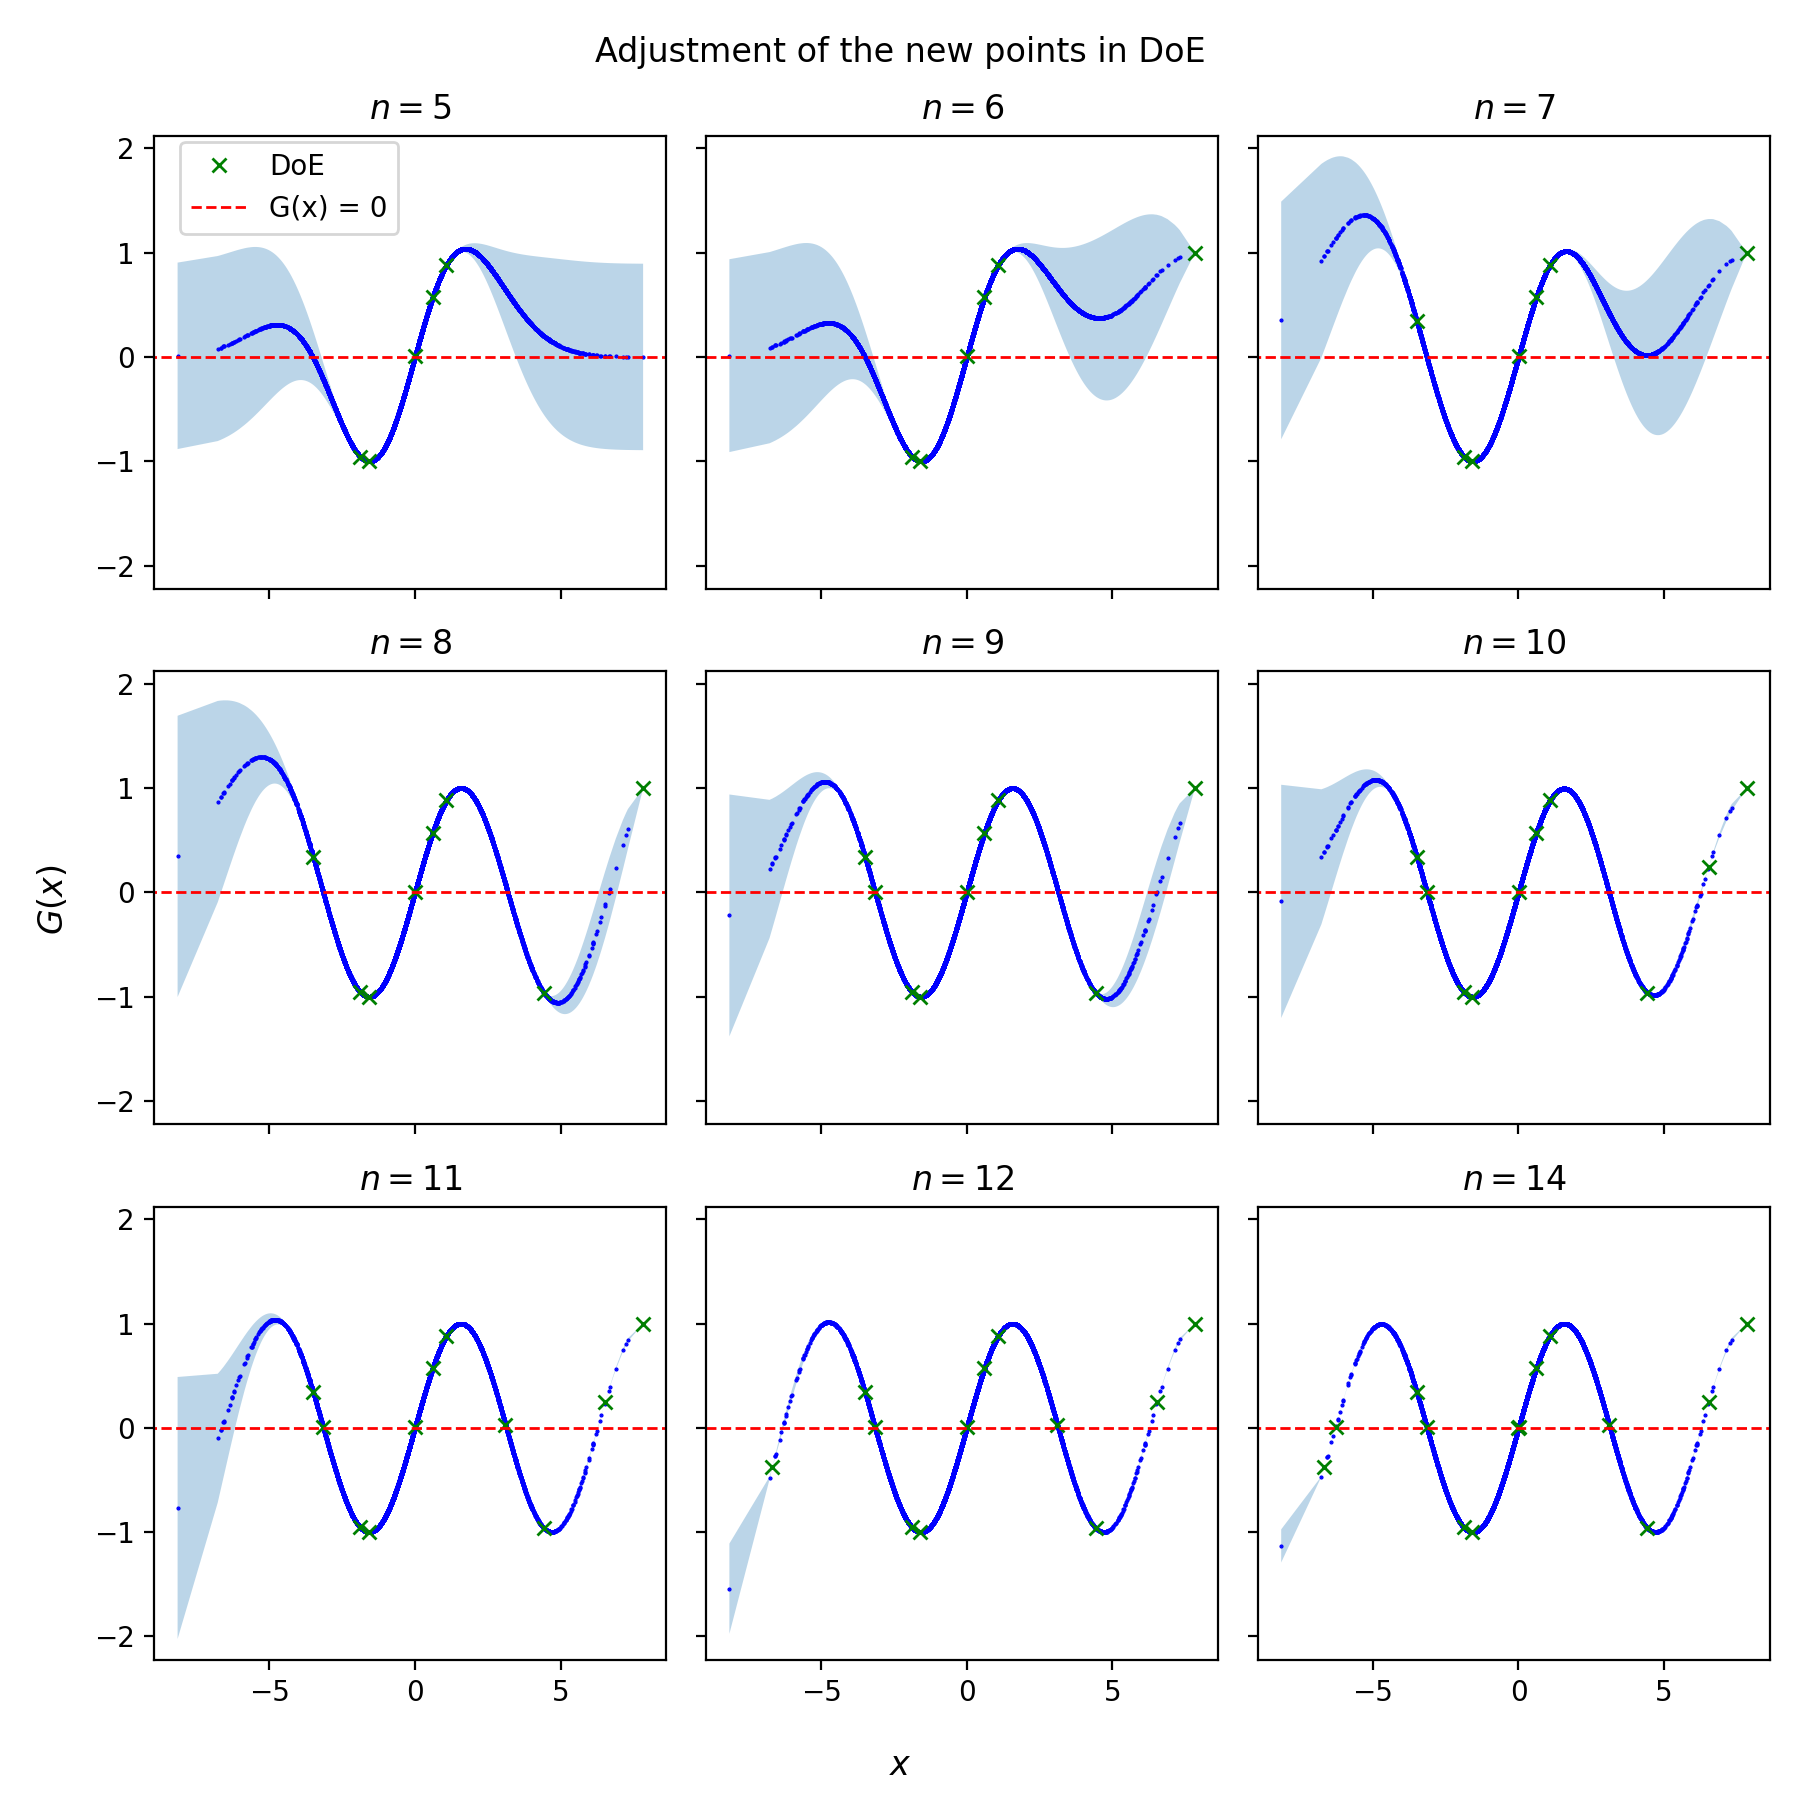
\includegraphics{1d_exa_1d.png}
    \caption{Prediction and standard deviation obtained with $n$ points
    in the DoE.}
    \label{fig:ex1}
\end{figure}

\begin{table}[h]
  \footnotesize%
  \begin{center}
  \begin{tabular}{lclcc}
  \toprule
  Method & $N_{call}$  & $\widehat{p_f}$ $(\text{C.O.V}_{\widehat{p_f}})$ &$\epsilon_{\widehat{p_f}}(\%)$  \\
  \midrule
  Monte Carlo   & \num[round-precision=1,round-mode=figures]{10000} & \num{0.4944}($1.01\%$) & - \\
  AK-MCS+U & $14$ & \num{0.4944} & $0$ \\
  \bottomrule
  \end{tabular}
  \end{center}
  \caption{Results of example 1}
  \label{tab:res_ex1}
\end{table}

In figure \ref{fig:ex1} it can be seen how the algorithm selects the next point to
be added to the DoE such that it reduces the most the variance near to the limit 
$G(\bm{x}) = 0$. Even though there is still some considerable variance in some regions,
it stops at $N = 14$ because this uncertainty is away from the limit, so it is
unlikely to affect the estimation of the probability of failure.
In fact, the results in table \ref{tab:res_ex1} reveal that a very accurate estimation
is obtained.

\subsection{Example 2: series system with four branches}
Taken from
\citep{Echard2011}. Both random variables
are standard normal distributed. The performance function is:
\begin{equation}
    G(x_1, x_2) = \text{min}
    \left\lbrace
    \begin{array}{c@{}l}
      3 + 0.1(x_1-x_2)^2 - \frac{(x_1+x_2)}{\sqrt{2}}; \\
      3 + 0.1(x_1-x_2)^2 + \frac{(x_1+x_2)}{\sqrt{2}}; \\
      (x_1-x_2) + \frac{4}{\sqrt{2}}; \\
      (x_2-x_1) + \frac{4}{\sqrt{2}}
    \end{array}
    \right\rbrace
  \end{equation}
with $k$ taking two different values: $6$ and $7$.

From the results on tables \ref{tab:res_ex2} and \ref{tab:res_ex2_2} we can see
that the learning function U obtained the most accurate estimations of $\widehat{p_f}$,
being exactly the same of the MCS. In the case $k=6$, the other two functions performed
well, they only failed at clasifying one point. In the other one, with $k=7$, EFF made some
misclassifications, but the learning function H, although calling the performance function
less times, had an error of $30\%$. \\

\begin{table}[h]
    \footnotesize
    \begin{center}
    \begin{tabular}{lclc}
    \toprule
    Method & $N_{call}$  & $\widehat{p_f}$ $(\text{C.O.V}_{\widehat{p_f}})$ &$\epsilon_{\widehat{p_f}}(\%)$  \\
    \midrule
    Monte Carlo   & \num[round-precision=1,round-mode=figures]{1000000} & \num{0.004433}($1.5\%$) & - \\
    AK-MCS+U & $126$ & \num{0.004433} & $0$ \\
    AK-MCS+EFF & $123$ & \num{0.004432} & $0.02$ \\
    AK-MCS+H & $113$ & \num{0.004434} & $0.02$ \\
    \bottomrule
    \end{tabular}
    \end{center}
    \caption{Results of example 2 with $k=6$}
    \label{tab:res_ex2}
\end{table}

\begin{table}[h]
    \footnotesize
    \begin{center}
    \begin{tabular}{lclc}
    \toprule
    Method & $N_{call}$  & $\widehat{p_f}$ $(\text{C.O.V}_{\widehat{p_f}})$ &$\epsilon_{\widehat{p_f}}(\%)$  \\
    \midrule
    Monte Carlo   & \num[round-precision=1,round-mode=figures]{1000000} & \num{0.002161}($2.15\%$) & - \\
    AK-MCS+U & $103$ & \num{0.002161} & $0$ \\
    AK-MCS+EFF & $107$ & \num{0.002156} & $0.23$ \\
    AK-MCS+H & $65$ & \num{0.0015} & $30.59$ \\
    \bottomrule
    \end{tabular}
    \end{center}
    \caption{Results of example 2 with $k=7$}
    \label{tab:res_ex2_2}
\end{table}

In the figure \ref{fig:ex2_mc} the actual distribution of the two classes in the
MC population is displayed, while in the figure \ref{fig:ex2_iteru} there is the
distribution predicted by AK-MCS+U at several stages. Additionally, figure \ref{fig:ex2_iteru}
give some insights about the update of the DoE, showing how the selected points tend to
come from near the limit $G(\bm{x}) = 0$. \\

\begin{marginfigure}
    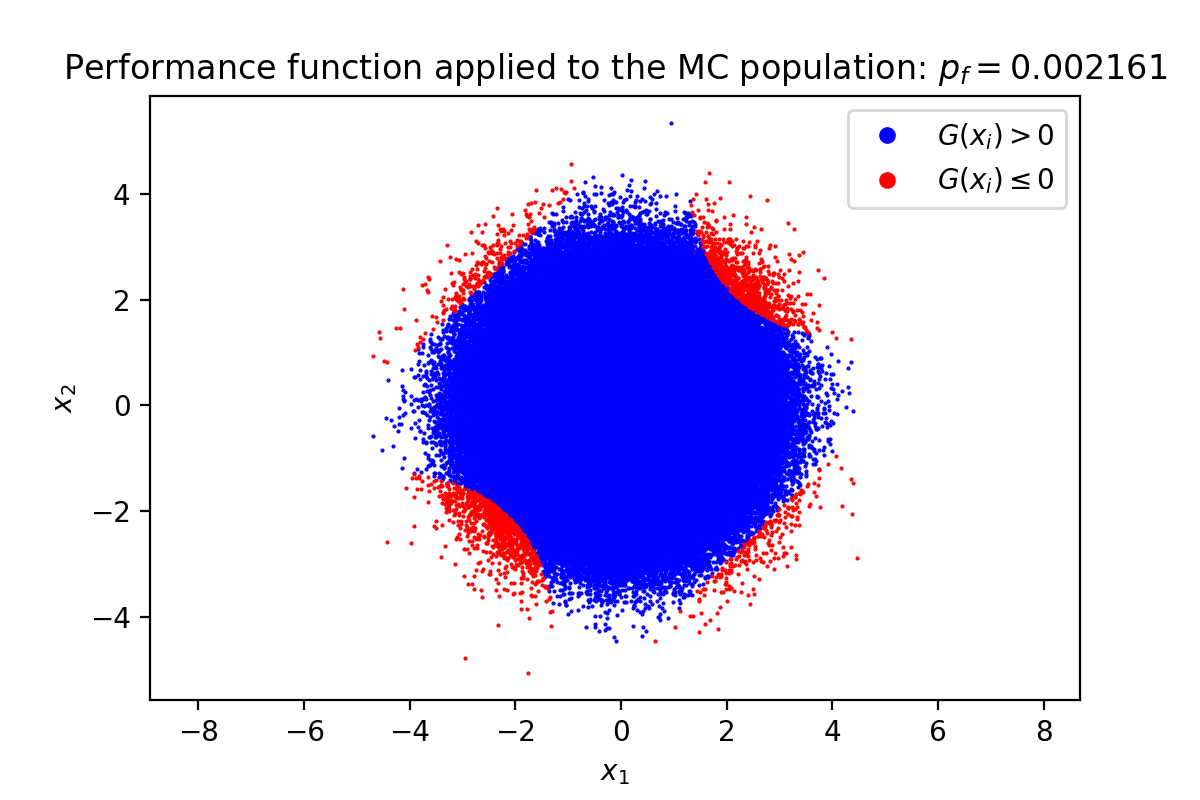
\includegraphics[width=\linewidth]{mc_ex_2D_k7.png}
    \caption{Example 2 with $k=7$. Evaluation of the performance function on the MC population.}
    \label{fig:ex2_mc}
\end{marginfigure}

\begin{figure*}[h!]
    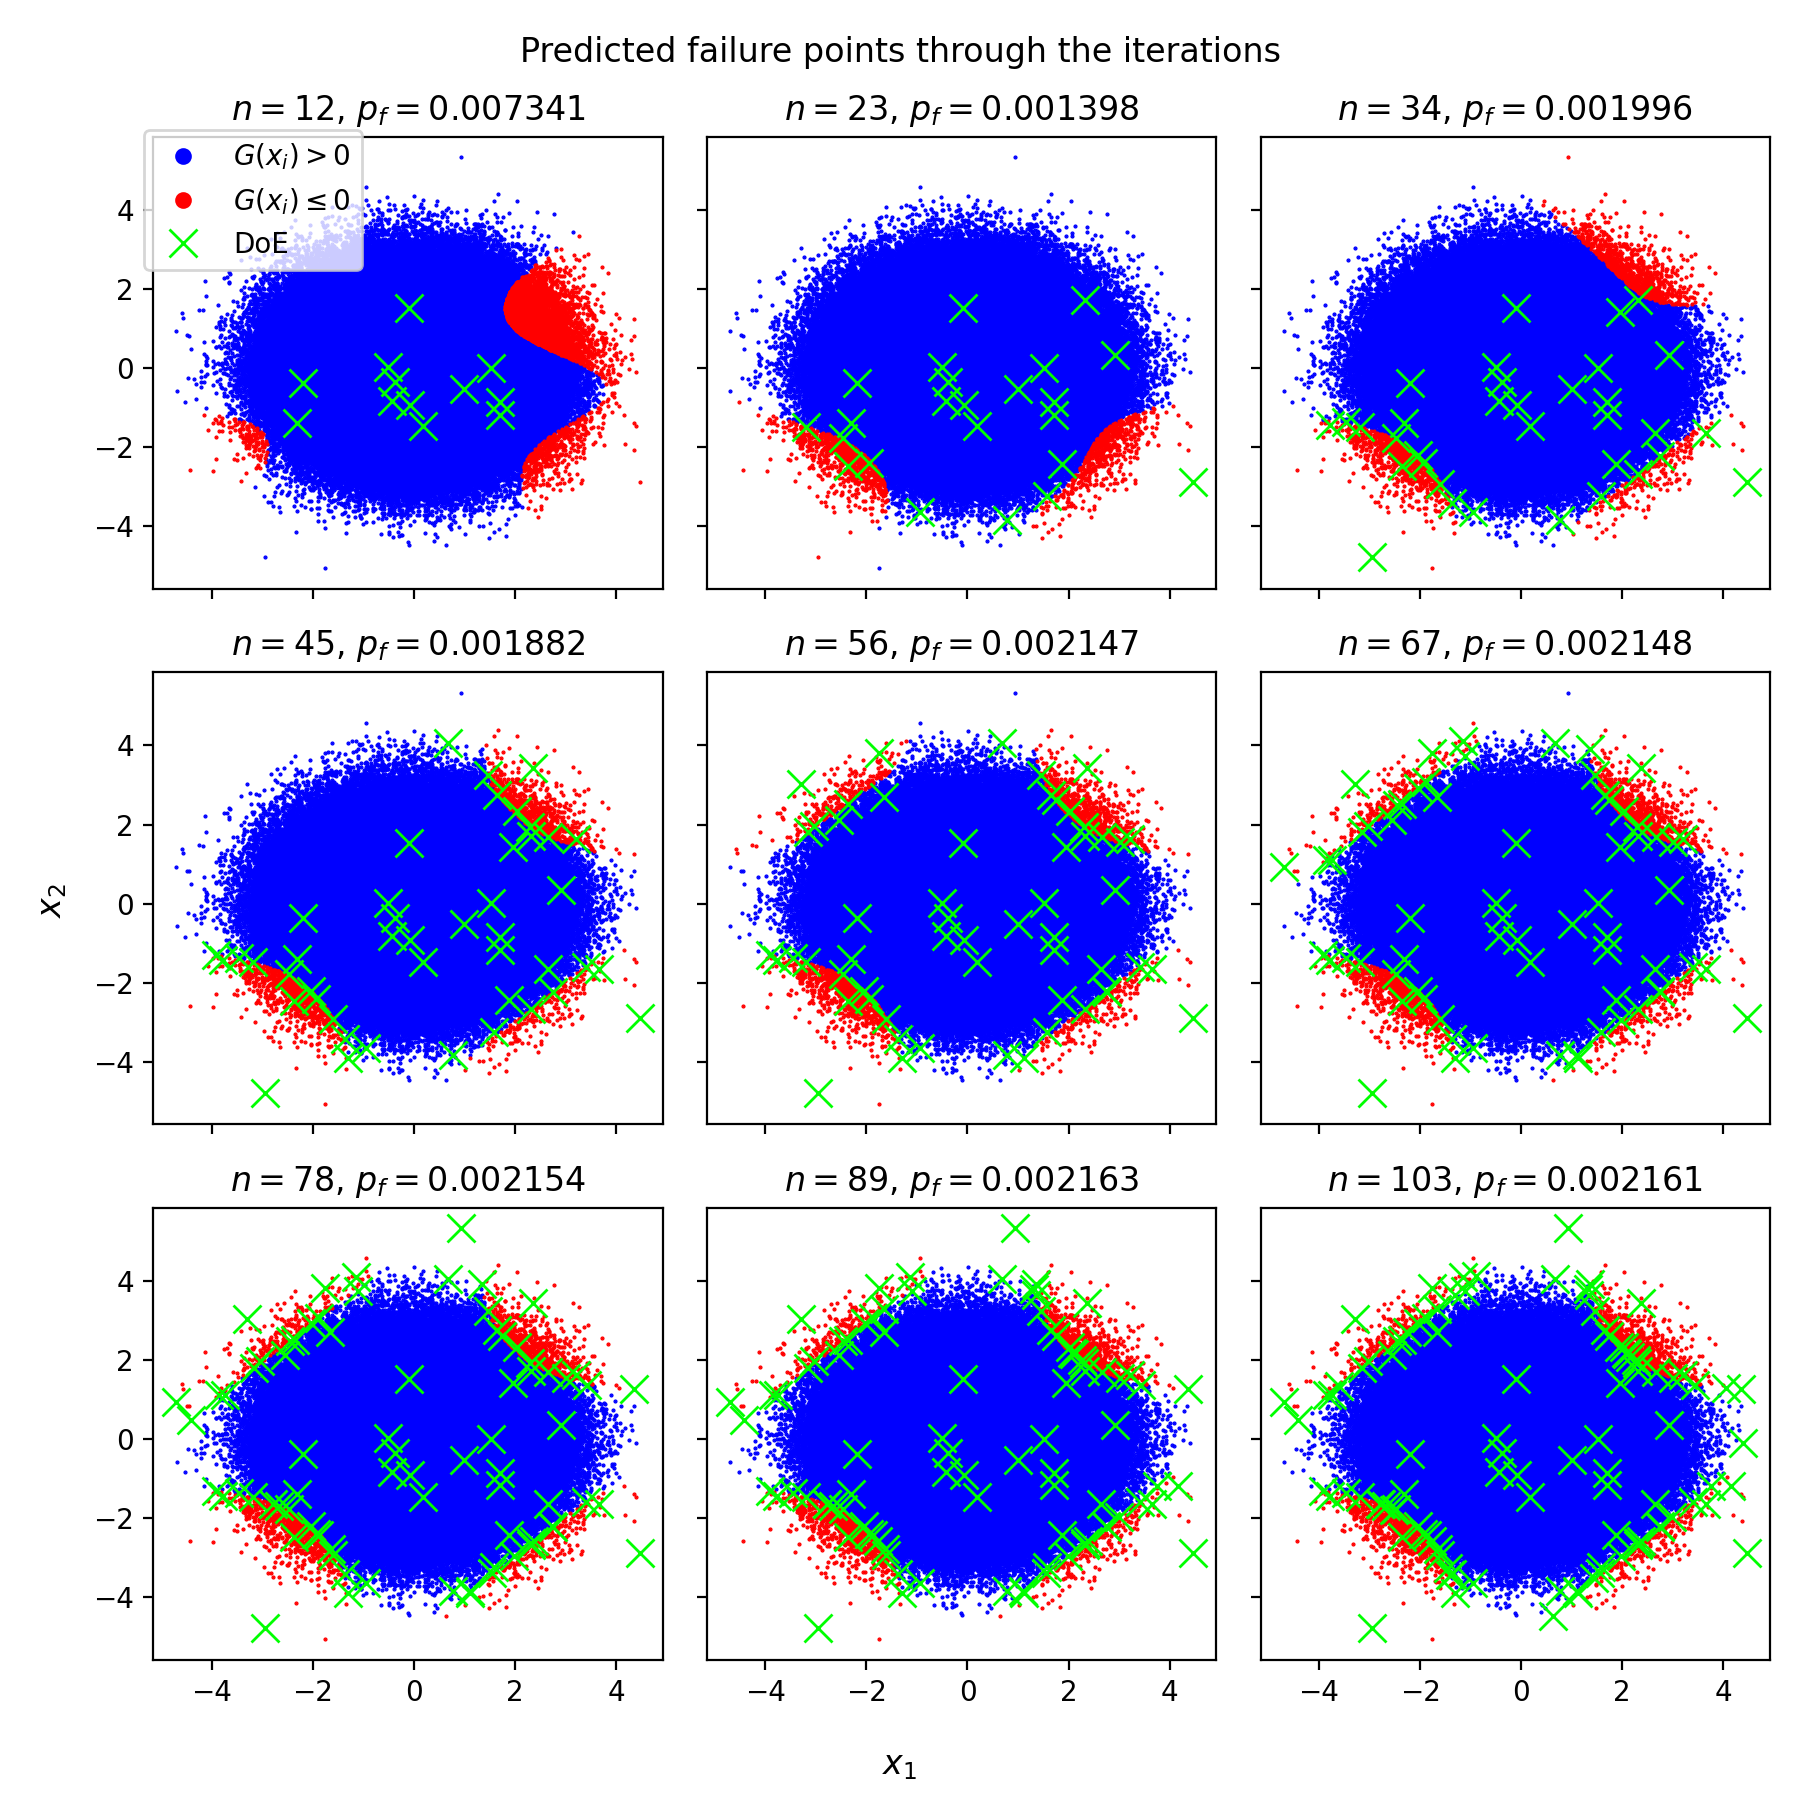
\includegraphics{iter_ex_2D_k7_U.png}
    \caption{Example 2 with $k=7$. Prediction made by AK-MCS+U at several stages.}
    \label{fig:ex2_iteru}
\end{figure*}

Figures  \ref{fig:ex2_k6} and \ref{fig:ex2_k7} display how the probability of failure
converges with each learning function, and how the selected points make the learning criteria
tend to the stopping conditions. In both cases there are similar behaviors. The 
EFF is proned to converge more consistently to the stopping condition. The function 
U usually gets a good estimation well before finishing. The function H
presents the most irregular results. 

\begin{figure*}[h]
    \begin{subfigure}{.5\textwidth}
        \centering
        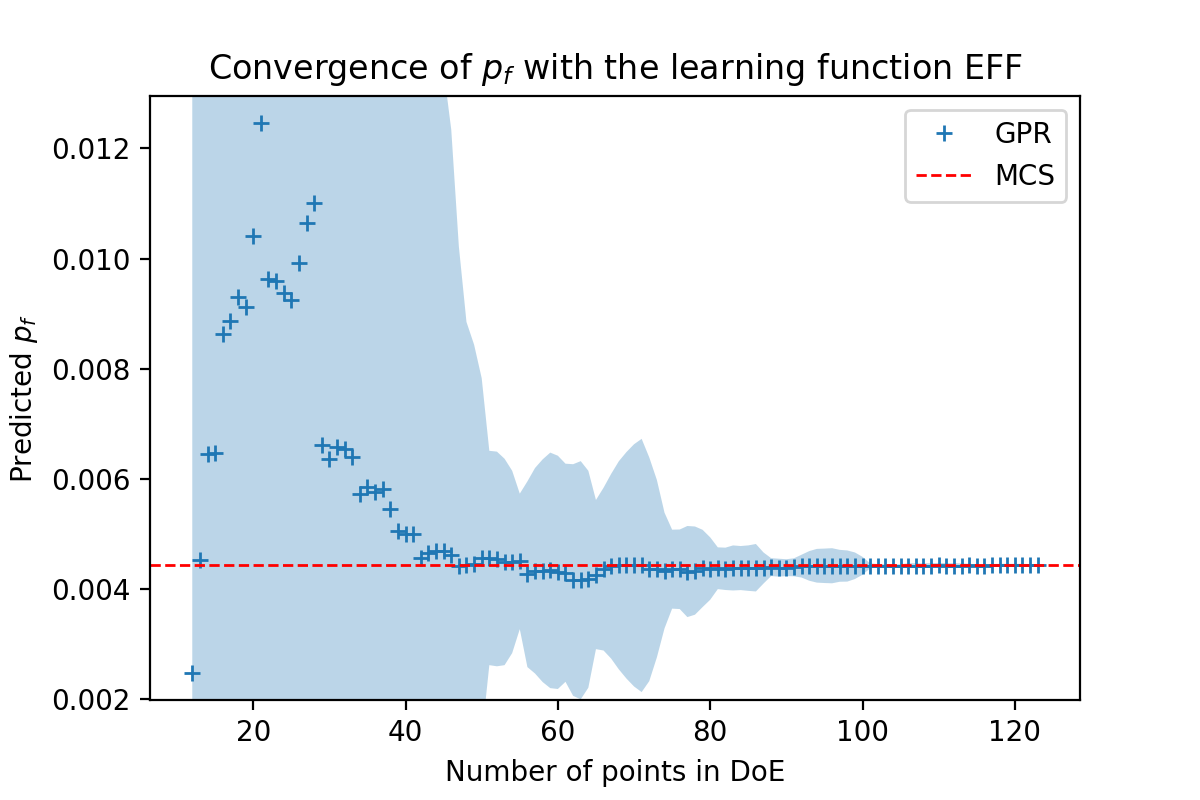
\includegraphics[width=\linewidth]{conv_ex_2D_k6_EFF.png}
      \end{subfigure}%
      \begin{subfigure}{.5\textwidth}
        \centering
        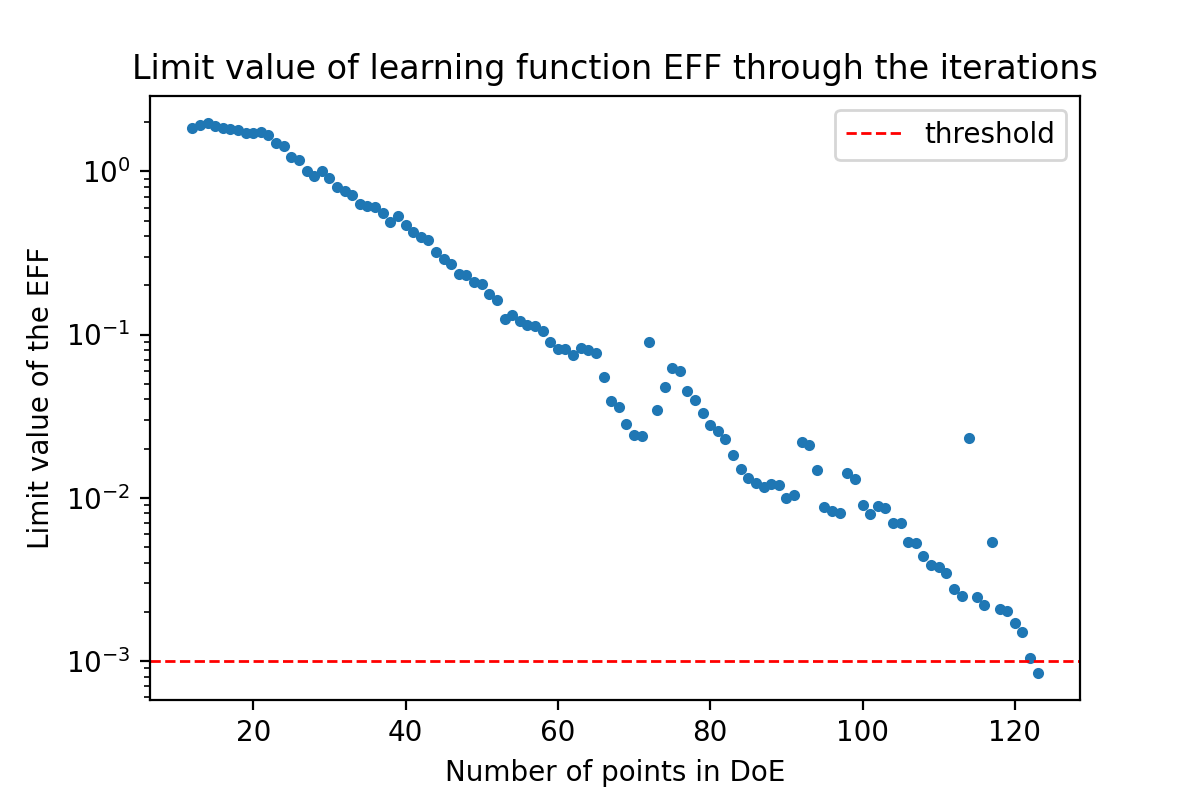
\includegraphics[width=\linewidth]{ex_2D_k6_EFF_lim_values.png}
      \end{subfigure}%
      \\
      \begin{subfigure}{.5\textwidth}
        \centering
        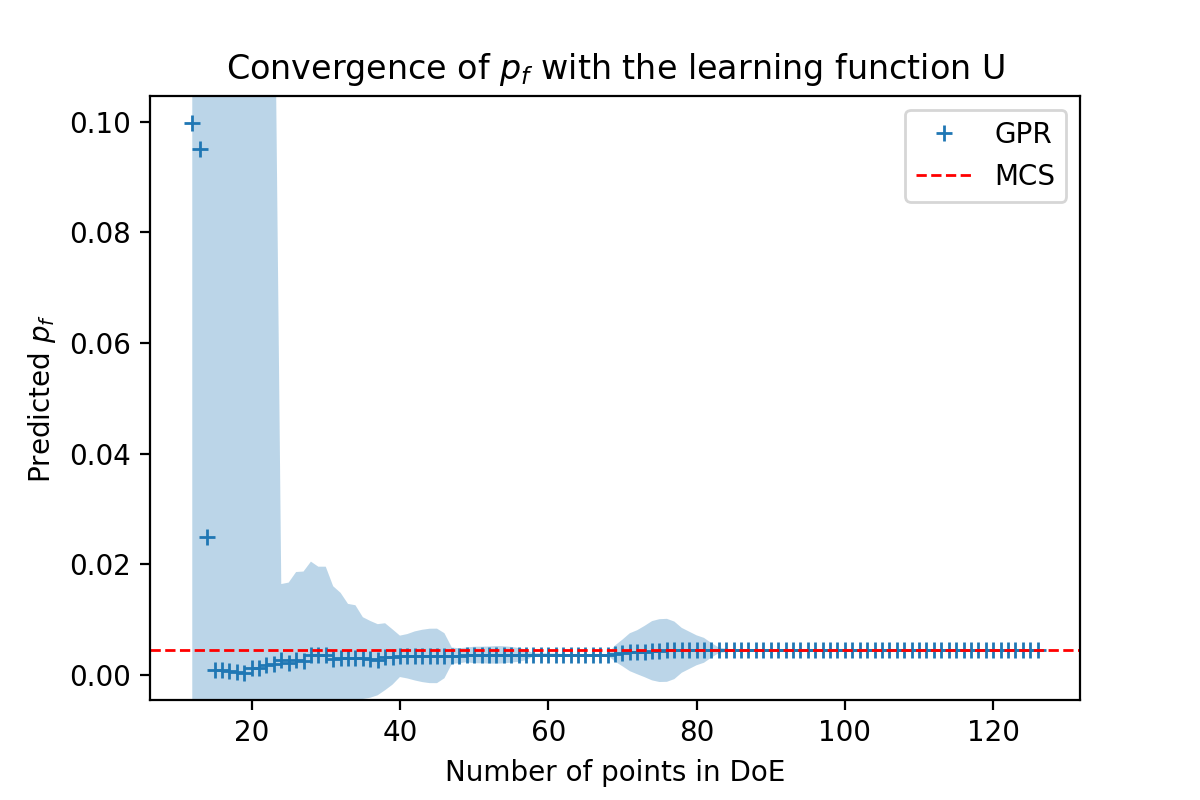
\includegraphics[width=\linewidth]{conv_ex_2D_k6_U.png}
      \end{subfigure}%
      \begin{subfigure}{.5\textwidth}
        \centering
        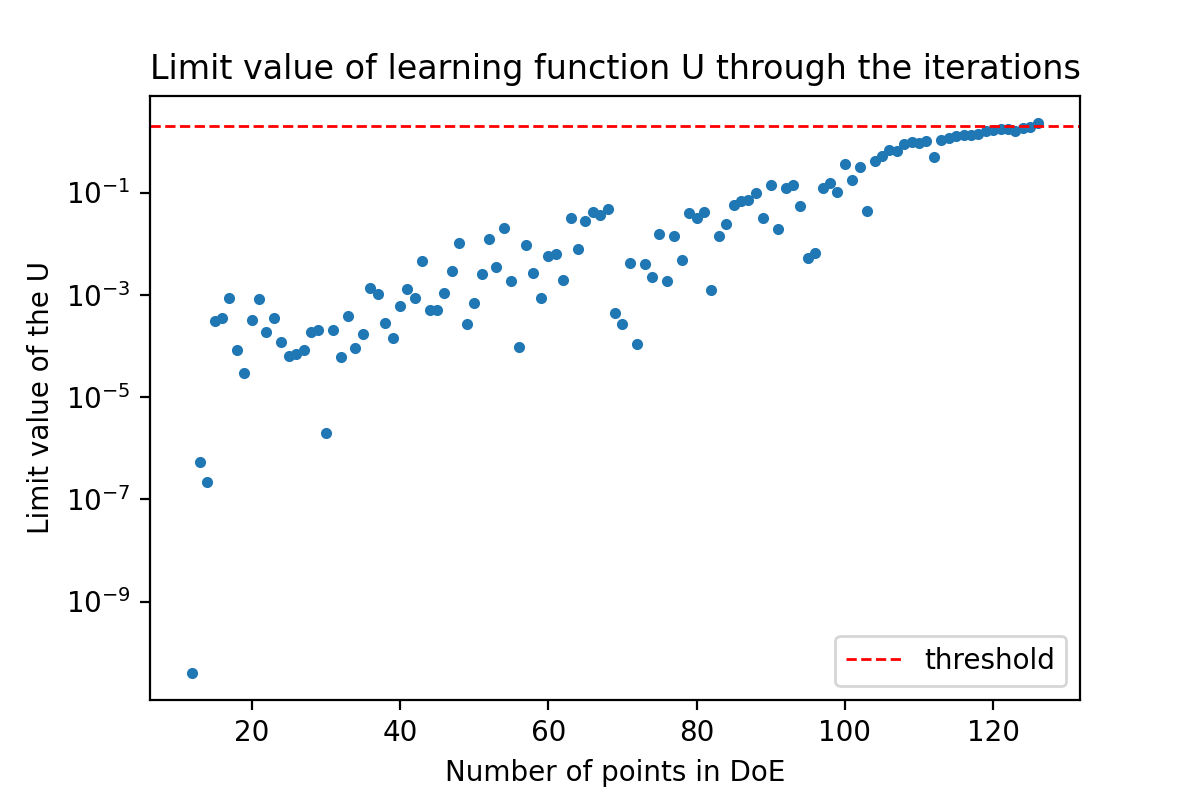
\includegraphics[width=\linewidth]{ex_2D_k6_U_lim_values.png}
      \end{subfigure}%
      \\    \begin{subfigure}{.5\textwidth}
        \centering
        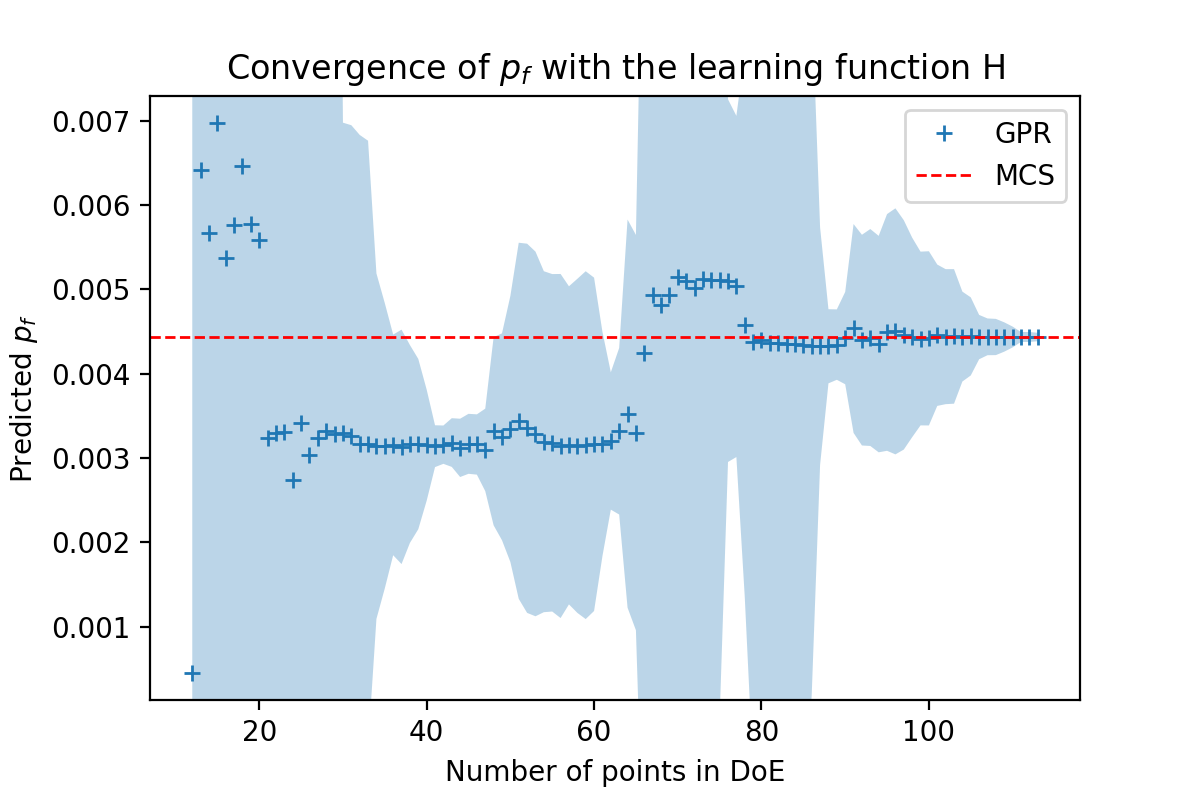
\includegraphics[width=\linewidth]{conv_ex_2D_k6_H.png}
      \end{subfigure}%
      \begin{subfigure}{.5\textwidth}
        \centering
        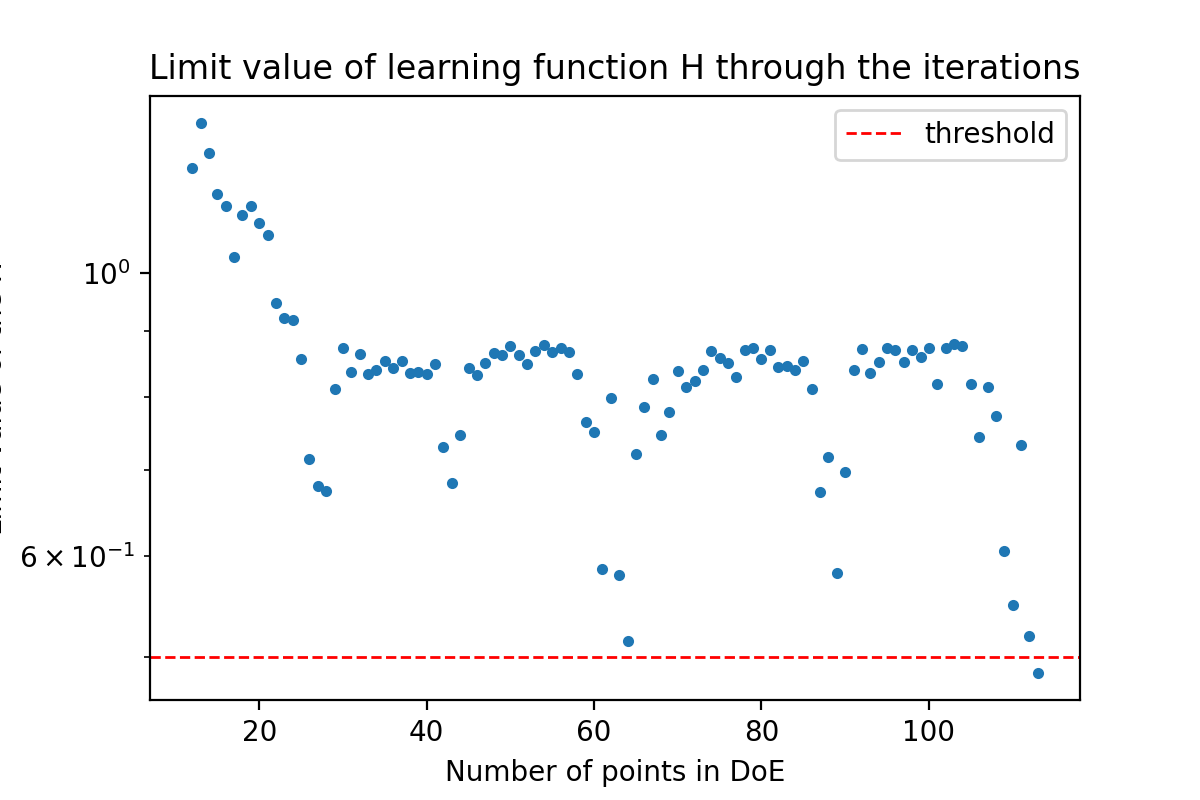
\includegraphics[width=\linewidth]{ex_2D_k6_H_lim_values.png}
      \end{subfigure}%
      \caption{Results of example 2 with $k=6$}
      \label{fig:ex2_k6}
\end{figure*}

\begin{figure*}[h]
    \begin{subfigure}{.5\textwidth}
        \centering
        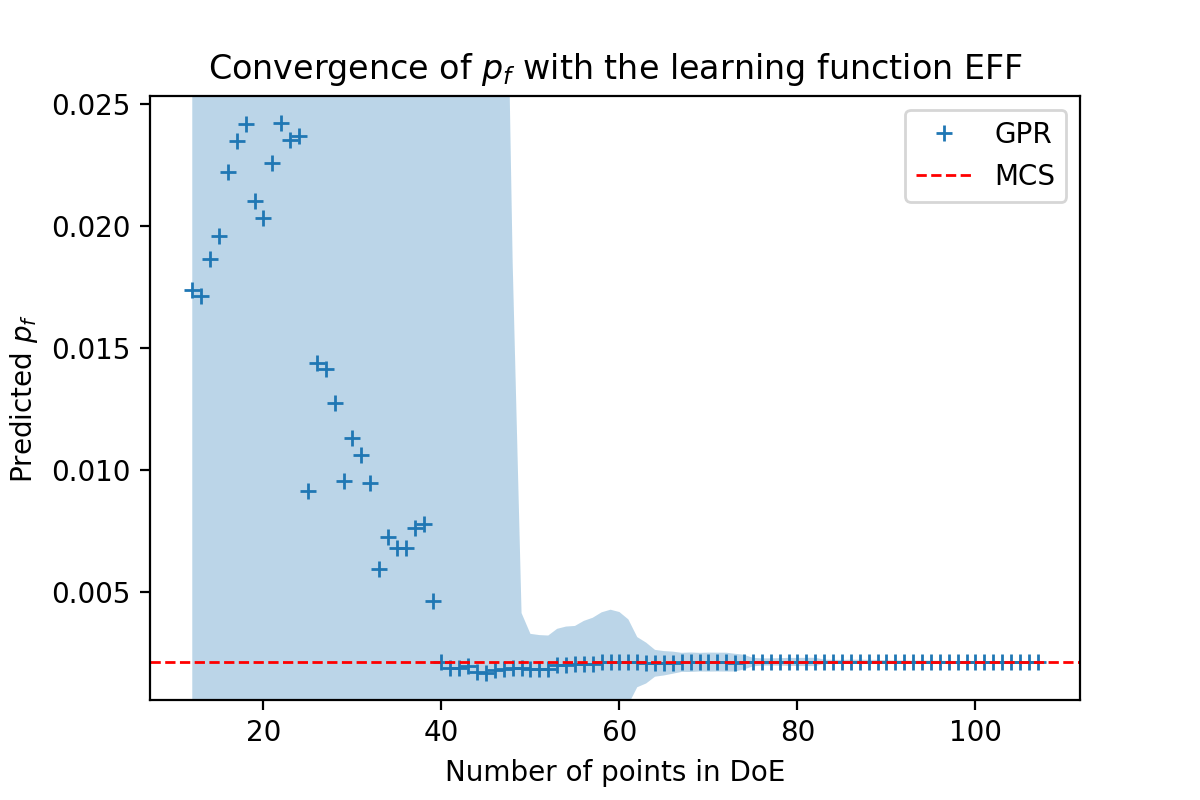
\includegraphics[width=\linewidth]{conv_ex_2D_k7_EFF.png}
      \end{subfigure}%
      \begin{subfigure}{.5\textwidth}
        \centering
        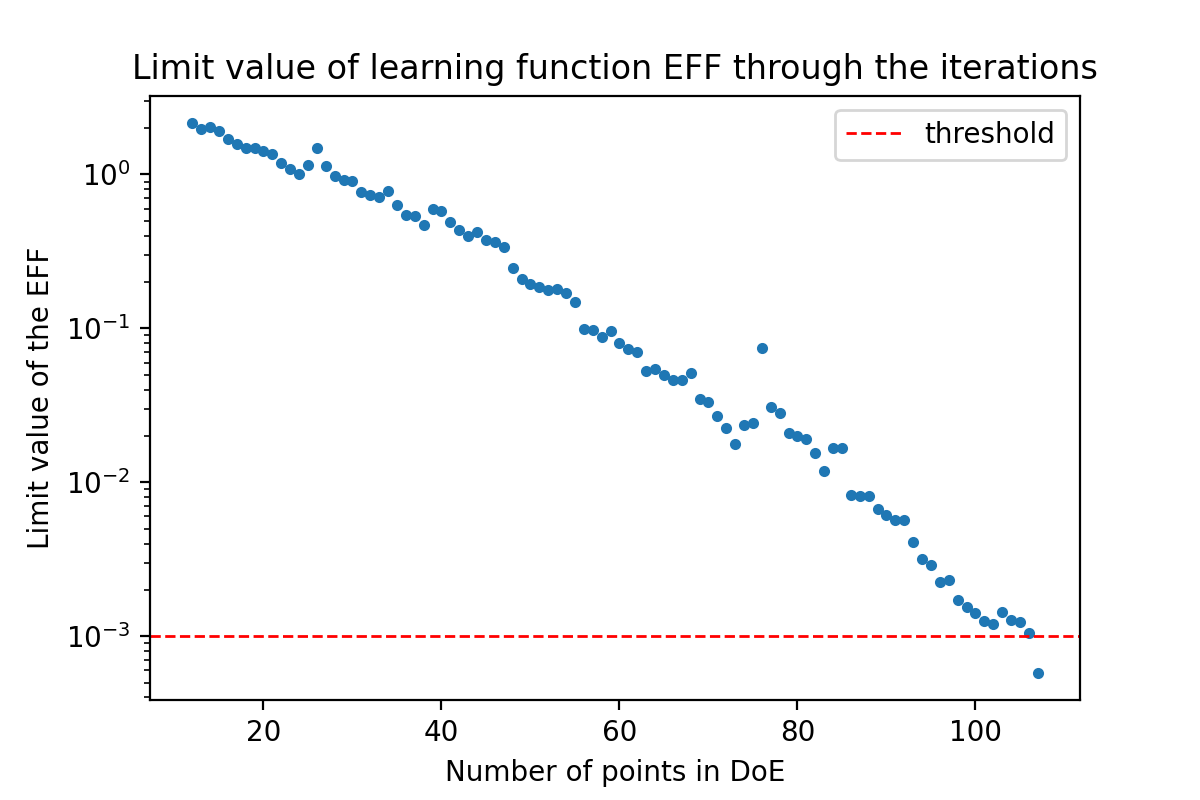
\includegraphics[width=\linewidth]{ex_2D_k7_EFF_lim_values.png}
      \end{subfigure}%
      \\
      \begin{subfigure}{.5\textwidth}
        \centering
        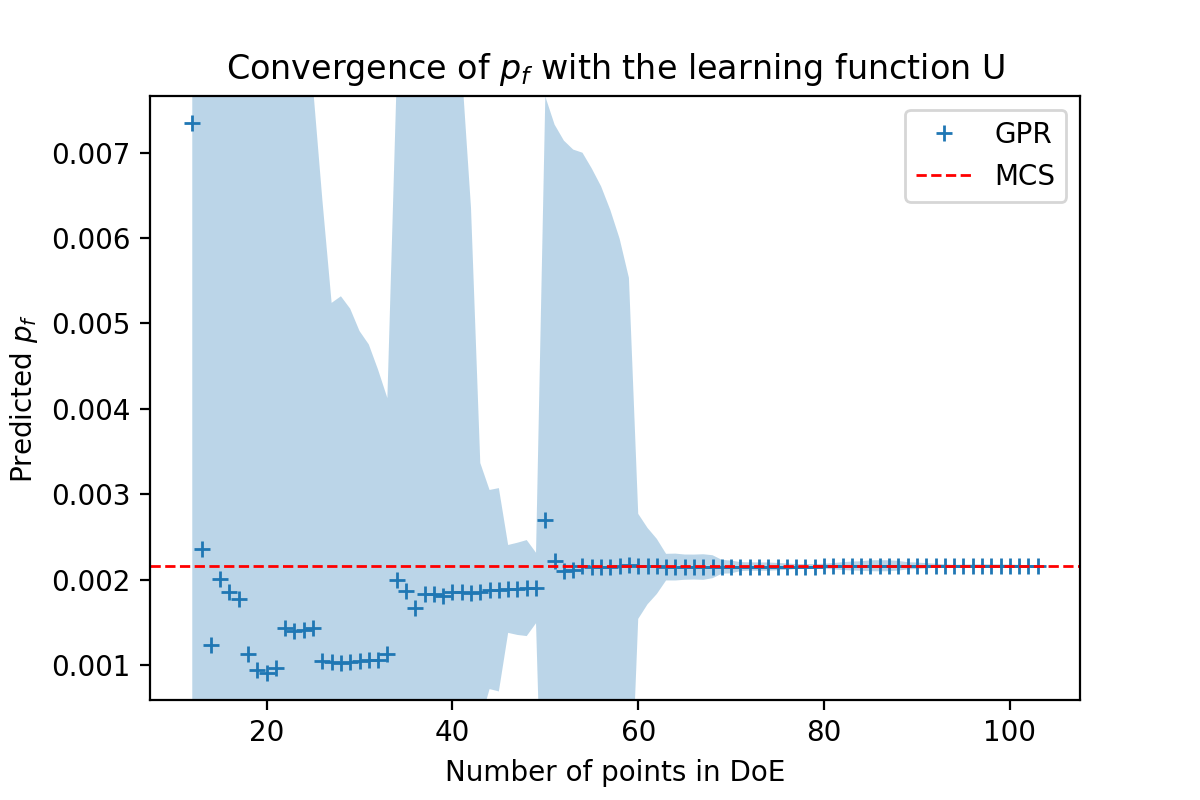
\includegraphics[width=\linewidth]{conv_ex_2D_k7_U.png}
      \end{subfigure}%
      \begin{subfigure}{.5\textwidth}
        \centering
        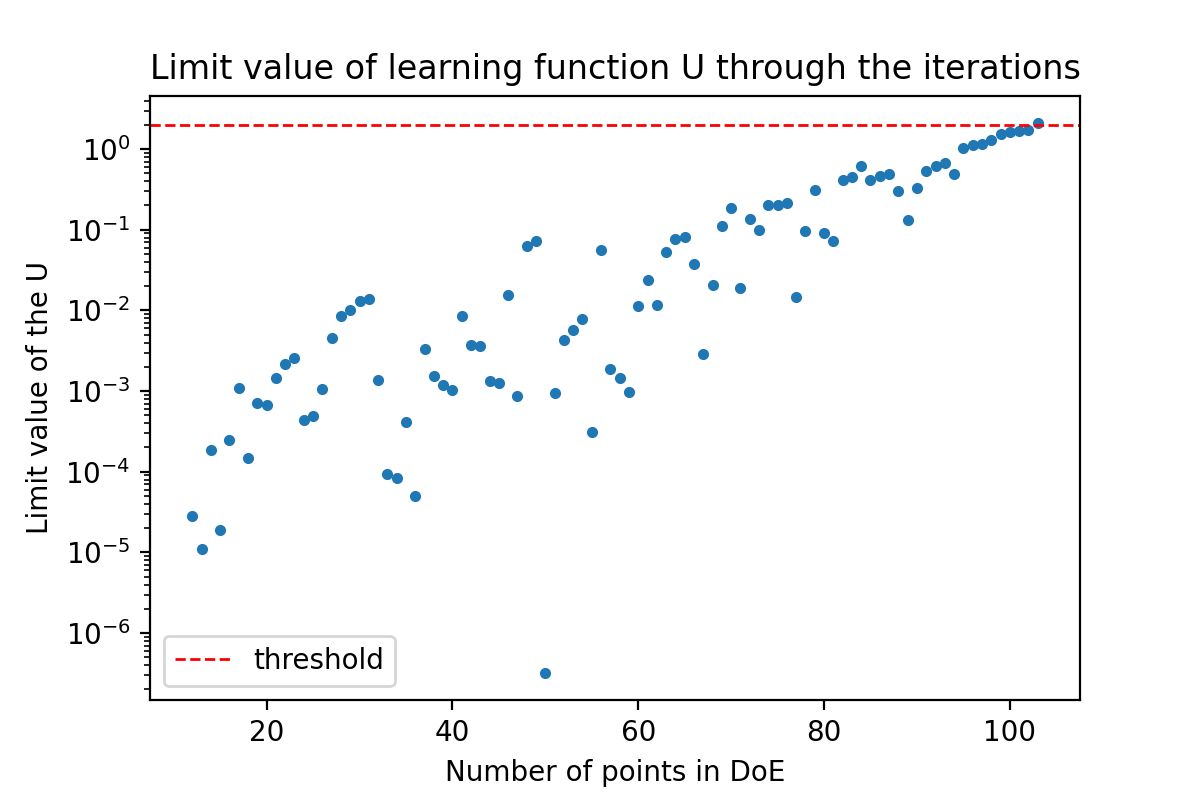
\includegraphics[width=\linewidth]{ex_2D_k7_U_lim_values.png}
      \end{subfigure}%
      \\    \begin{subfigure}{.5\textwidth}
        \centering
        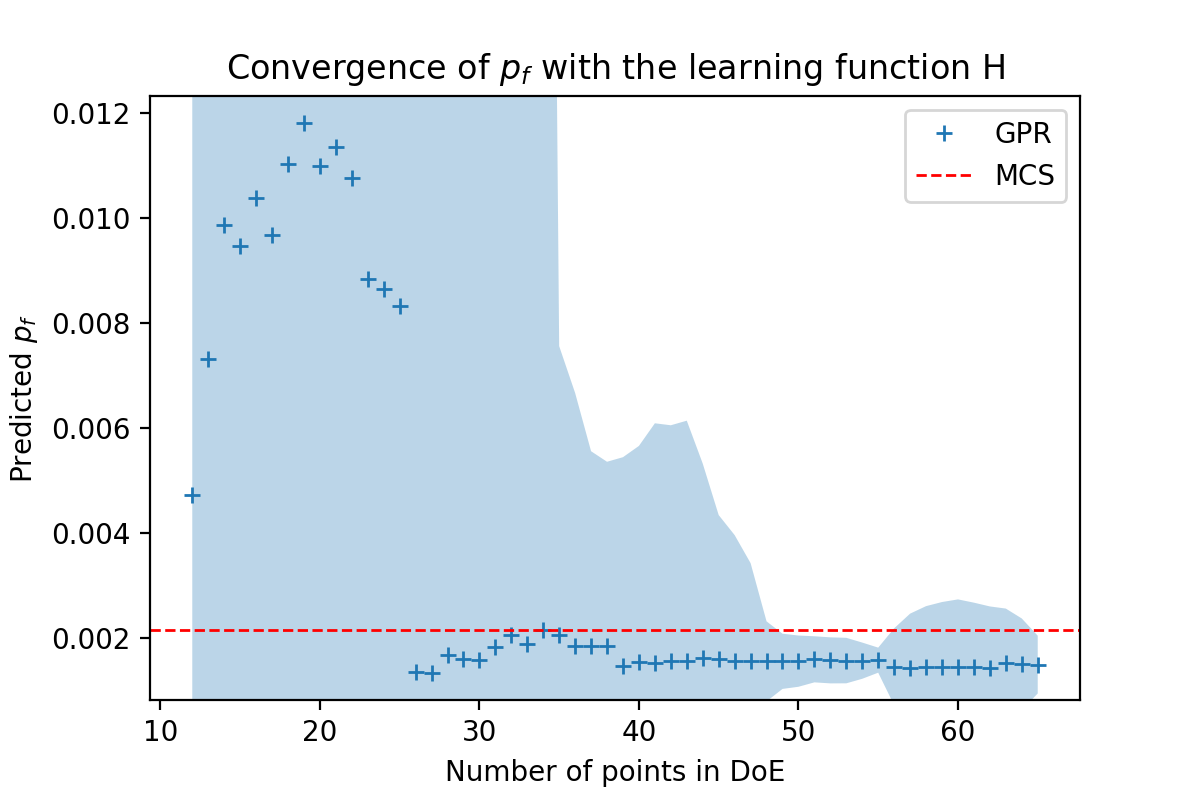
\includegraphics[width=\linewidth]{conv_ex_2D_k7_H.png}
      \end{subfigure}%
      \begin{subfigure}{.5\textwidth}
        \centering
        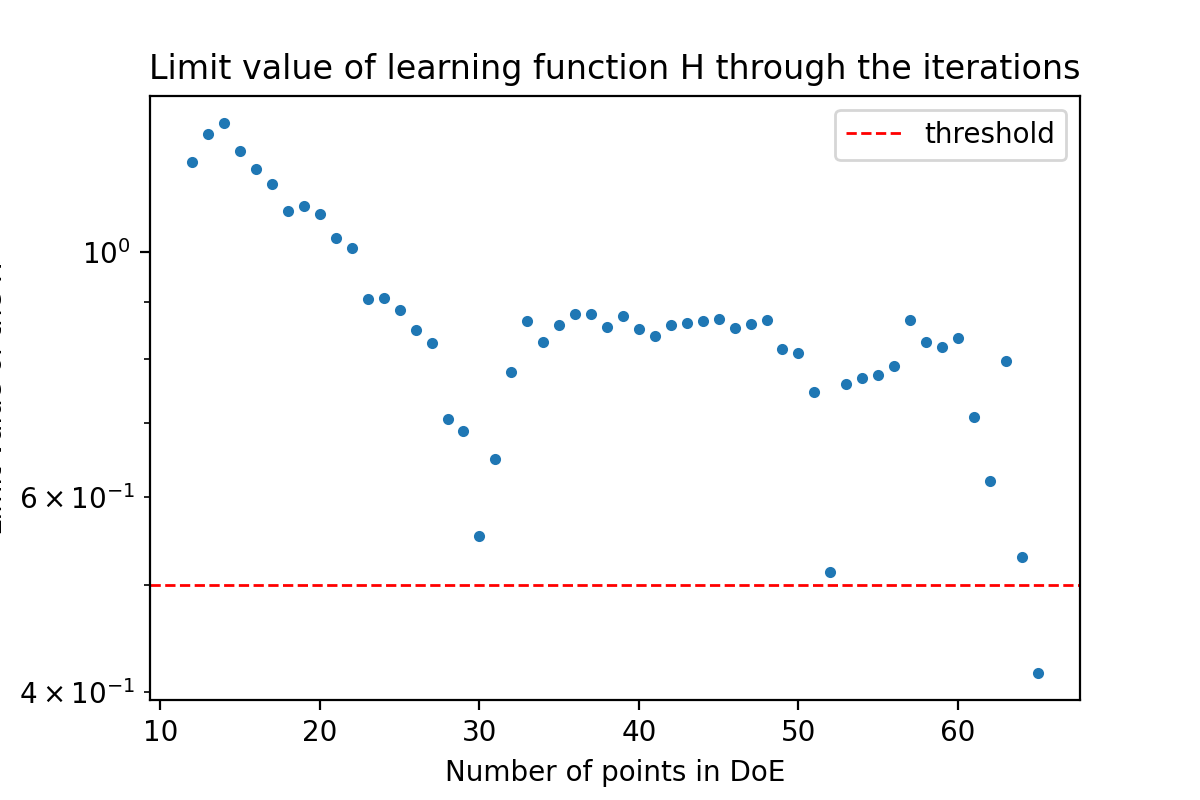
\includegraphics[width=\linewidth]{ex_2D_k7_H_lim_values.png}
      \end{subfigure}%
      \caption{Results of example 2 with $k=7$}
      \label{fig:ex2_k7}
\end{figure*}

\clearpage
\newpage
\subsection{Example 3: dynamic response of a non-linear oscillator}
Taken from \citep{Schueremans2005}. It is a non-linear undamped single degree of freedom system, as the
one shown in figure \ref{fig:ex3}. The involved variables are listed in table \ref{tab:var_ex3}.

\begin{equation}
  G(\pmb{x}) = 3r - \left\lvert\frac{2F_i}{m\omega_0^2} \sin{\paren{\frac{\omega_0 t_1}{2}}} \right\rvert
\end{equation}
where $\omega_0 = \sqrt{\frac{c_1 + c_2}{m}}$

\begin{figure}[h]
    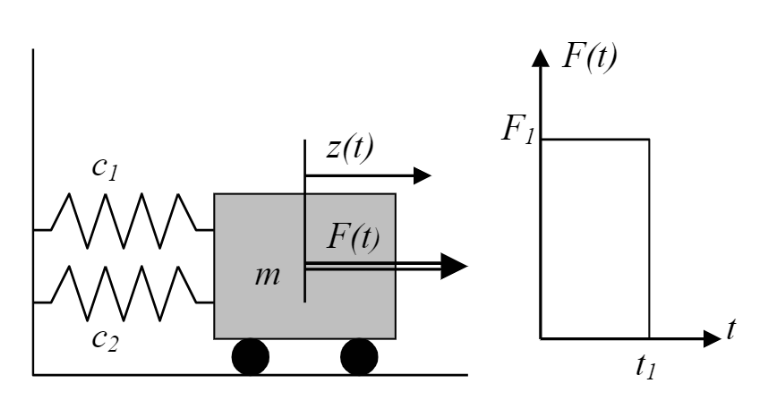
\includegraphics{ex_3.png}
    \caption{Example 3. Non-linear oscilator. Taken from \citep{Schu2005}}
    \label{fig:ex3}
\end{figure}

\begin{table}[h]
    \footnotesize%
    \begin{center}
    \begin{tabular}{cccc}
    \toprule
    Variable & P.D.F & Mean & Standard deviation \\
    \midrule
    $m$   & Normal & $1$ & $0.05$ \\
    $c_1$   & Normal & $1$ & $0.1$ \\
    $c_2$   & Normal & $0.1$ & $0.01$ \\
    $r$   & Normal & $0.5$ & $0.05$ \\
    $F_1$   & Normal & $1$ & $0.2$ \\
    $t_1$   & Normal & $1$ & $0.2$ \\
    \bottomrule
    \end{tabular}
    \end{center}
    \caption{Random variables of example 3}
    \label{tab:var_ex3}
\end{table}

Table \ref{tab:res_ex3} contains the obtained results. In contrast with the other
examples, in this case the function H performs quite well, obtaining the exact result, just
as the function U, but with some more calls to the performance function. \\

In figure \ref{fig:ex3_results} it is evident that the function EFF met its stopping
condition before converging to the solution, unlike the other two functions.

\begin{table}[h]
    \footnotesize
    \begin{center}
    \begin{tabular}{lclc}
    \toprule
    Method & $N_{call}$  & $\widehat{p_f}$ $(\text{C.O.V}_{\widehat{p_f}})$ &$\epsilon_{\widehat{p_f}}(\%)$  \\
    \midrule
    Monte Carlo   & \num[round-precision=1,round-mode=figures]{70000} & \num{0.027814}($2.23\%$) & - \\
    AK-MCS+U & $60$ & \num{0.027814} & $0$ \\
    AK-MCS+EFF & $43$ & \num{0.027671} & $0.51$ \\
    AK-MCS+H & $66$ & \num{0.027814} & $0$ \\
    \bottomrule
    \end{tabular}
    \end{center}
    \caption{Results of example 3}
    \label{tab:res_ex3}
\end{table}

\begin{figure*}[h]
    \begin{subfigure}{.5\textwidth}
        \centering
        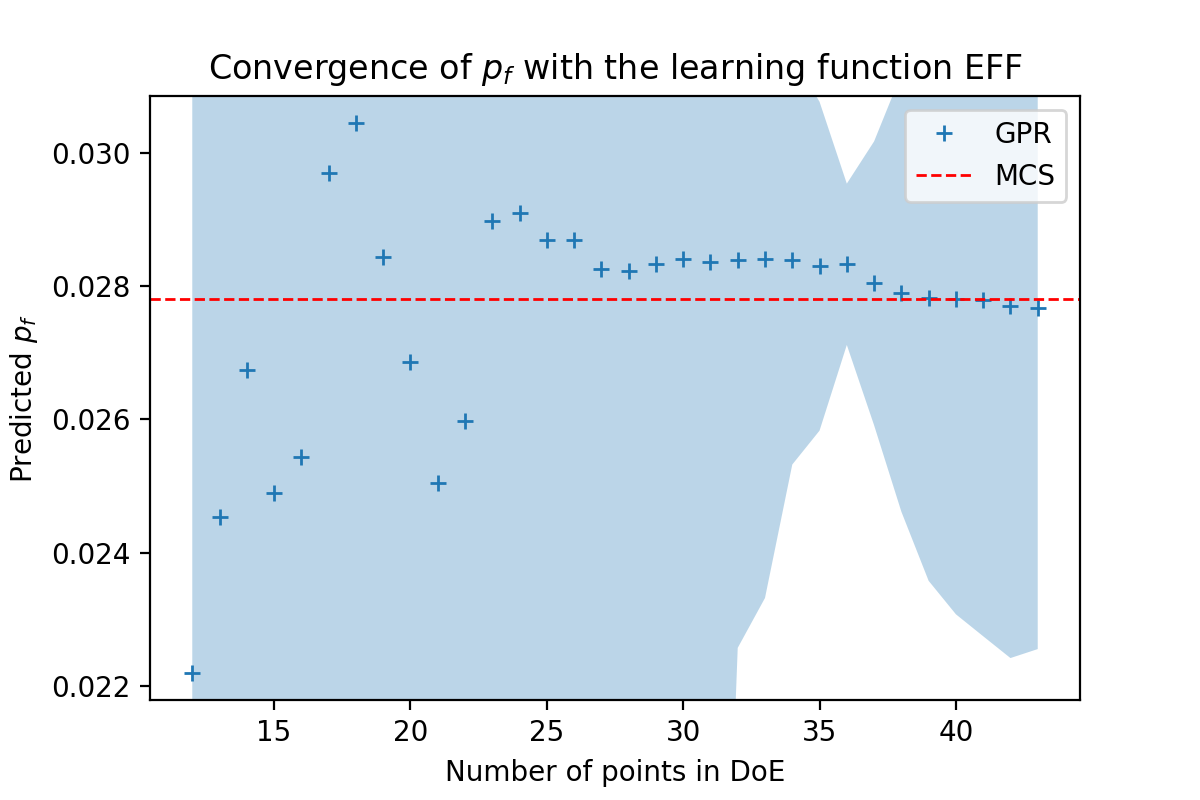
\includegraphics[width=\linewidth]{conv_ex_3_EFF.png}
      \end{subfigure}%
      \begin{subfigure}{.5\textwidth}
        \centering
        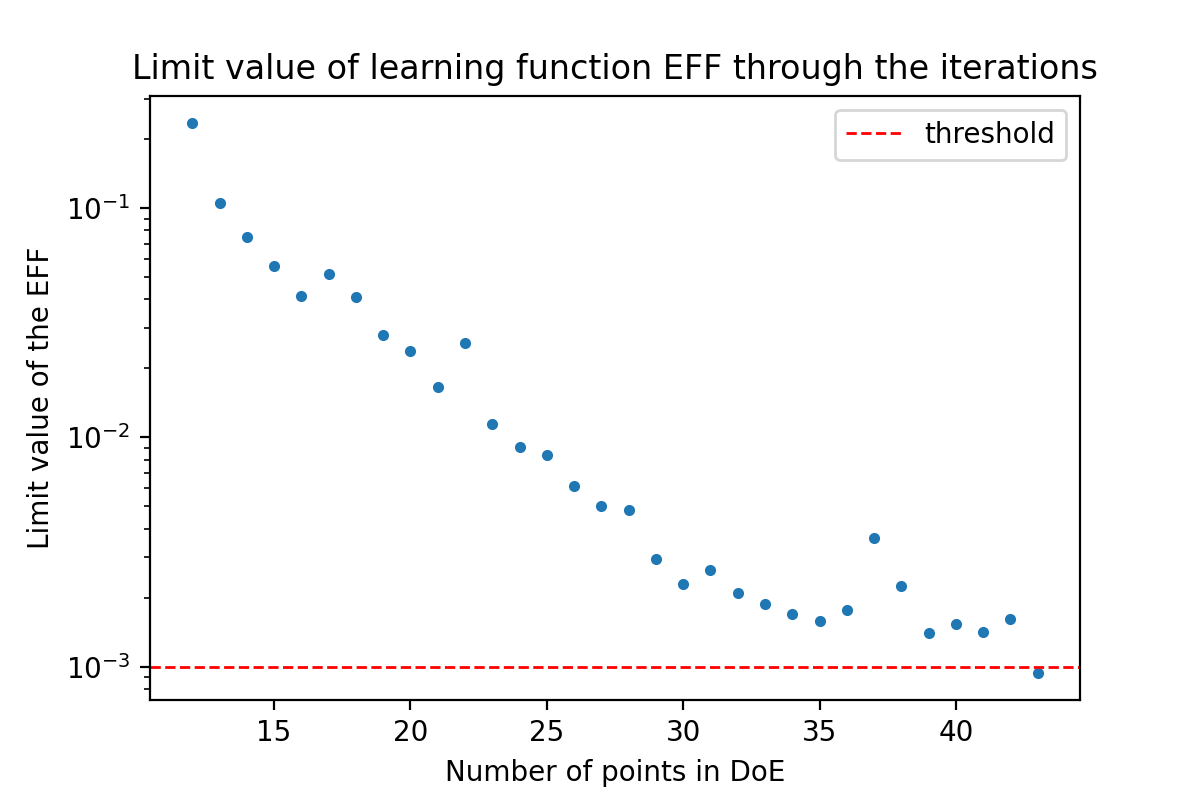
\includegraphics[width=\linewidth]{ex_3_EFF_lim_values.png}
      \end{subfigure}%
      \\
      \begin{subfigure}{.5\textwidth}
        \centering
        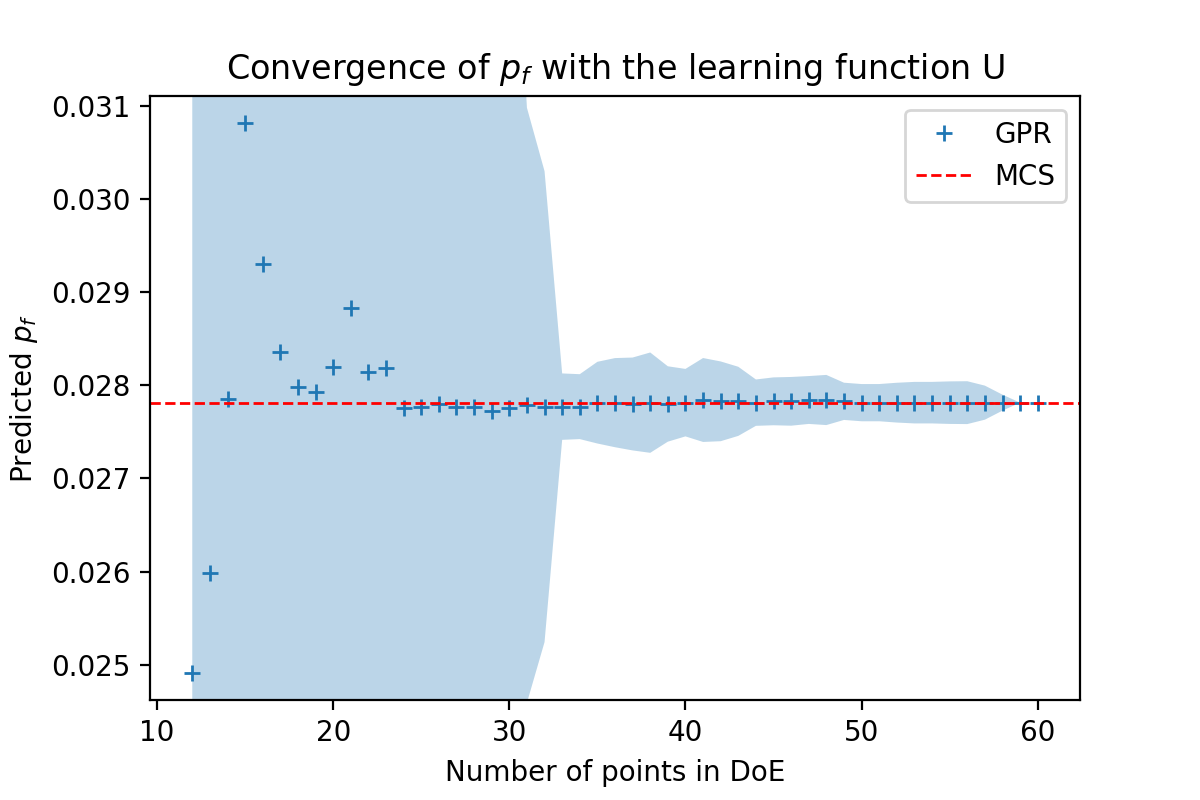
\includegraphics[width=\linewidth]{conv_ex_3_U.png}
      \end{subfigure}%
      \begin{subfigure}{.5\textwidth}
        \centering
        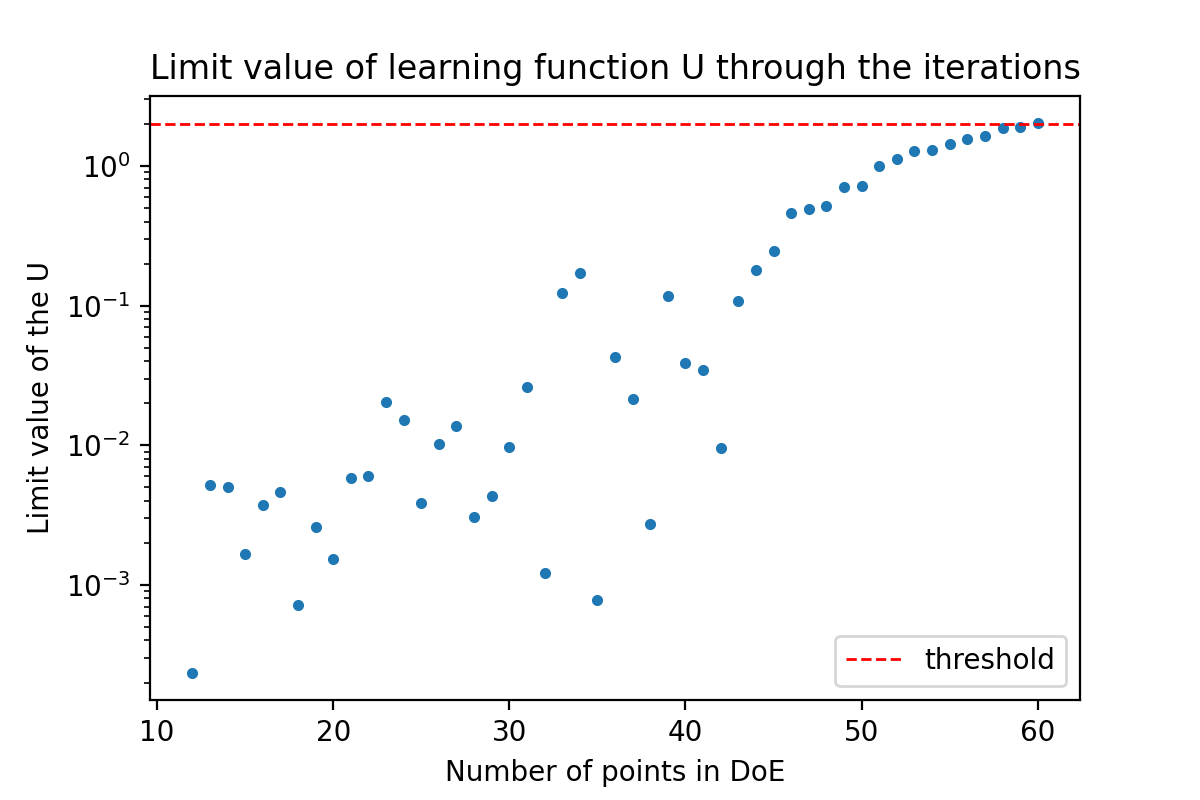
\includegraphics[width=\linewidth]{ex_3_U_lim_values.png}
      \end{subfigure}%
      \\    \begin{subfigure}{.5\textwidth}
        \centering
        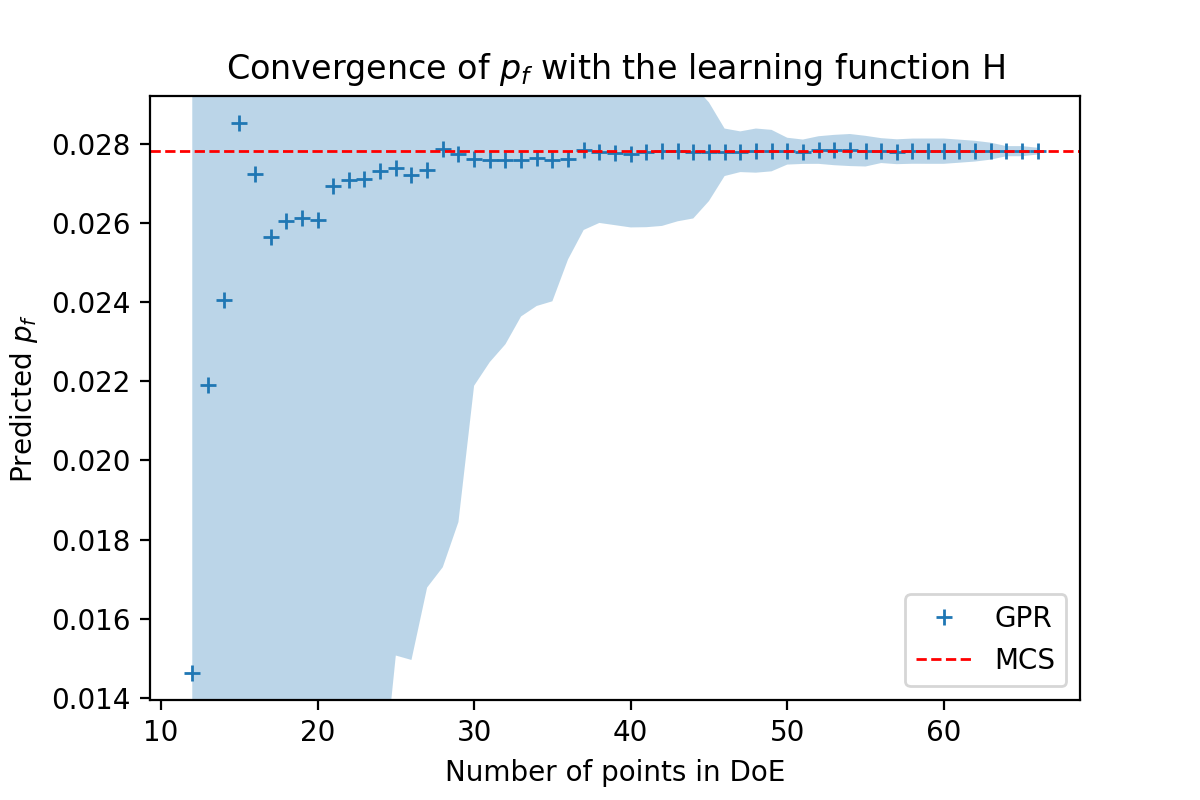
\includegraphics[width=\linewidth]{conv_ex_3_H.png}
      \end{subfigure}%
      \begin{subfigure}{.5\textwidth}
        \centering
        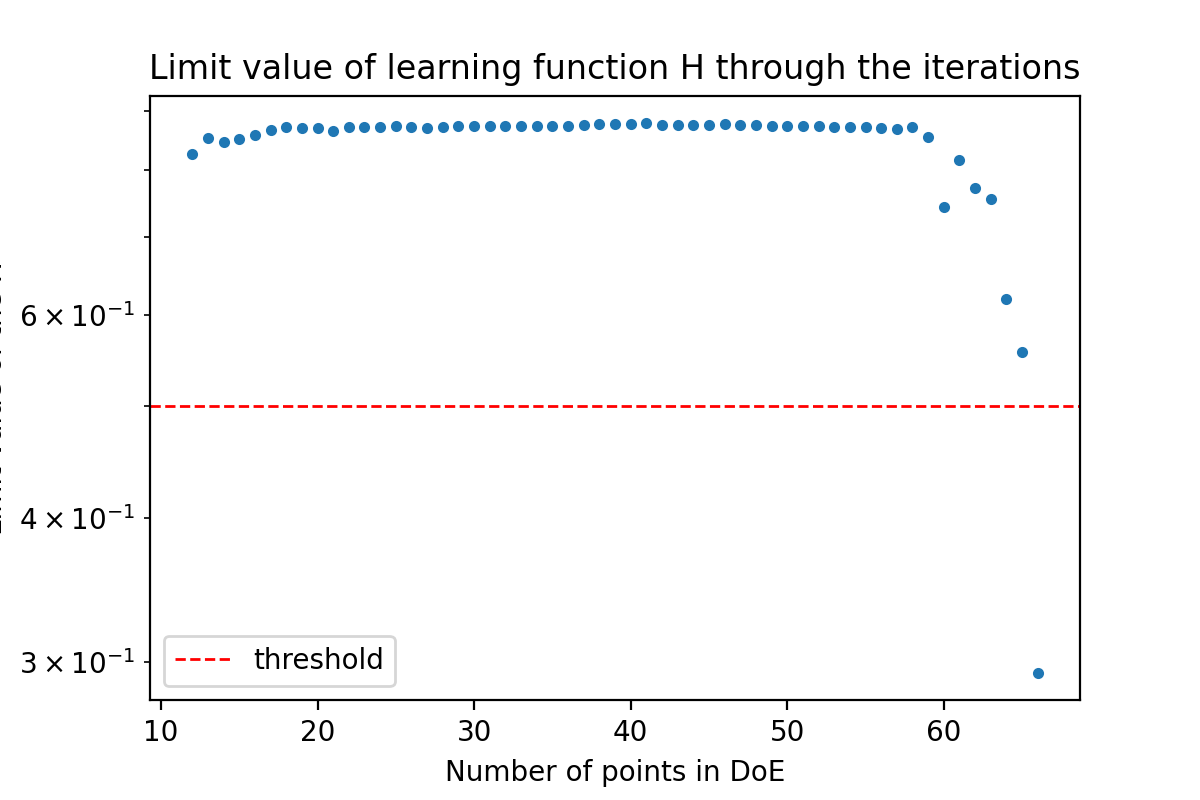
\includegraphics[width=\linewidth]{ex_3_H_lim_values.png}
      \end{subfigure}%
      \caption{Results of example 3}
      \label{fig:ex3_results}
\end{figure*}